\chapter{Experimentos}\label{cap.experimentos}
\hspace{1cm} En este cap\'itulo se van a comentar las distintas pruebas realizadas tanto con el drone real como en la simulaci\'on, las cuales validan cada fase del proyecto y la soluci\'on final. Tambi\'en estas pruebas han servido para depurar mientras se desarrollaba. 

\hspace{1cm} Para organizar las distintas pruebas, se va a hablar sobre la parte de percepci\'on. Tras esto se comentar\'a por separado cada una de las partes del algoritmo de navegaci\'on (despegue, b\'usqueda y aterrizaje), para terminar con una ejecuci\'on t\'ipica del algoritmo completo.

\hspace{1cm} En los experimentos realizados se han apreciado las diferencias importantes que hay entre trabajar en el entorno simulado y en el real. Primero, en el entorno simulado los colores son puros ideales y m\'as f\'aciles de detectar, sin embargo en el entorno real debido a luces y sombras un color puede verse m\'as o menos n\'itido, adem\'as de ser m\'as dif\'icil aislarlo del resto. Segundo, las velocidades a los motores a aplicar sobre uno y otro son distintas, pues en el entorno simulado se le puede dar una mayor velocidad que trabajar\'a sin problemas. Por el contrario, en el real una velocidad alta y un movimiento brusco puede llevar a desestabilizarlo. Tercero, en el drone real interviene tambi\'en el factor de la bater\'ia, en funci\'on de la carga que tuviera \'esta el drone aterrizaba con m\'as o menos fuerza y realizaba movimientos m\'as o menos fluidos. A partir del 30\% de bater\'ia no permit\'ia al drone realizar todos los movimientos, y en algunas ocasiones perd\'ia altura, aunque despu\'es volv\'ia a ganarla. 

\hspace{1cm} Los experimentos reales se han realizado con 3 ArDrone2 de Parrot distintos, entre los que se han apreciado comportamientos distintos pese a ser el mismo modelo del mismo fabricante. Se debe a que alguno ten\'ia mas deriva que los otros o que los movimientos eran mas bruscos seg\'un el drone.


\section{Percepci\'on de la baliza}\label{sec:percepcion}
%%QUE OBJETO DETECTAR???
\hspace{1cm} Para las pruebas de esta secci\'on hay que tener en cuenta que objeto detectar. Es un cuadrado con cuatro cuadrados dentro, dos de color naranja, y otros dos de color azul (trabajando con el drone real) o verde (si se trabajaba en un entorno simulado). 

%\hspace{1cm} Los primeros test se realizaban en el entorno simulado, al principio detectando ambos colores y viendo que se trataba de 4 objetos distintos. Despu\'es se comenzaron los test con el algoritmo final, viendo que los cuatro cuadrados formaban una cruceta y detectaba \'esta en la imagen, para as\'i poder centrarse. Dependiendo de los distintos estados del algor\'itmo, cuando ve\'ia una parte de la baliza la detectaba y marcaba como posible objeto, en caso de tratarse de la baliza completa la marcaba como tal. 


\hspace{1cm} Para verificar el funcionamiento de los filtros de color se realizaron tests en los cuales se detectaban por separado los colores de la baliza y se contaba el n\'umero de objetos. Para verificar que los objetos que se detectaban eran la baliza deseada, se pasaba por dos fases. Para una posible baliza, se marcaba el objeto en el interfaz gr\'afico. En caso de que se detectara la cruceta de los 4 cuadrados, se señalaba \'esta sobre la imagen y la baliza completa, como muestra la figura \ref{f:Deteca_objeto}.

\begin{figure}[H]
 \centering
  \subfloat[Percepci\'on posible objeto]{
   \label{f:Posible objeto}
    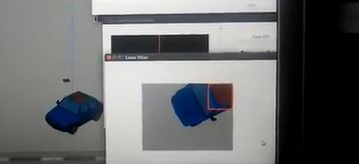
\includegraphics[width=0.4\textwidth]{imgs/perception1.jpg}}
  \subfloat[Detecta objeto]{
   \label{f: Deteca_objeto}
    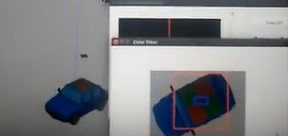
\includegraphics[width=0.4\textwidth]{imgs/perception2.jpg}} 
 \caption{Drone detectando objeto en escenario simulado.}
 \label{f:Drone detecta objeto. }
\end{figure} 

%\hspace{1cm} Una vez se realizaron \'estos con \'exito, pasaron a realizarse las pruebas con el drone real. Las primeras pruebas eran con el drone quieto y situando las balizas en distintas posiciones y viendo que las detectaba. Tras esto con el drone volando se hicieron pruebas, viendo que cuando se situaba la baliza debajo de este era capaz de detectarla. 

\hspace{1cm} Para realizar las pruebas en un entorno real se pon\'ia el drone en una posici\'on fija y se iba moviendo la baliza sobre distintas posiciones de la c\'amara y viendo si las detectaba o no. Para observar lo que detectaba se marcaba en la interfaz gr\'afica en color azul el centro de la cruceta y con rojo los posibles objetos, coincidiendo con la baliza completa, como muestra la figura \ref{fig:Detectando_baliza_real}.

\begin{figure}[H]
	\centering
		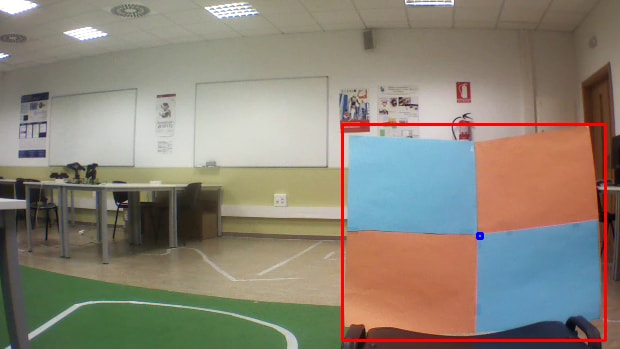
\includegraphics[width=0.55\textwidth]{imgs/k_beacon21.jpg}
		\caption{Detectando baliza real.}
	\label{fig:Detectando_baliza_real}
\end{figure}


\hspace{1cm} La parte de la percepci\'on es satisfactoria, pues se ha conseguido una detecci\'on robusta. Apenas hay falsos negativos(no detectar una baliza existente), y tampoco falsos positivos(detectar como baliza algo que no lo es). Adem\'as, el algoritmo se ha probado en diferentes ambientes con distinta luminosidad. Es importante tambi\'en el tipo de baliza elegida a detectar, ya que es un objeto dif\'icil de confundir con otros.


\section{Despegue}

%\hspace{1cm} Las primeras pruebas del despegue sobre el simulador fueron las mas sencillas. Esto se debe a que se trata de un entorno ideal en el cual el drone no tiene deriva ni se dan otros factores externos. Las pruebas consist\'ian en despegar el drone y que este se centrara sobre la baliza, aunque tambi\'en se prob\'o a despegar el drone sobre el coche con la baliza y mover el coche para ver que el drone le iba siguiendo. Esta parte se decidi\'o implementar porque el drone ten\'ia una deriva que le llevaba a desplazarse hacia atr\'as cuando ten\'ia que estar en el sitio. Cuando se hicieron las primeras pruebas de esto, se vi\'o que el drone siempre despegaba en esta direcci\'on y hab\'ia un dos segundos en los que no se pueden controlar sus movimientos, por tanto hab\'ia que contar con este desplazamiento.

\hspace{1cm} Para verificar el despegue en un entorno simulado, las pruebas que se realizaron fueron fructiferas (figuras \ref{fig:Despegue sobre la baliza del coche} y \ref{f:Test Despegue}). Esto se debe a que se trata de un entorno ideal en el cual el drone no tiene deriva ni se dan otros factores externos como las turbulencias. Las pruebas consist\'ian en despegar el drone y que \'este se centrara sobre la baliza, y despegar el drone sobre el coche con la baliza y mover el coche para ver que el drone le iba siguiendo. De este modo se probaba la capacidad de mantener al drone m\'as o menos centrado sobre la baliza de despegue.% Esta parte se decidi\'o implementar porque el drone real ten\'ia una deriva que le llevaba a desplazarse hacia atr\'as cuando ten\'ia que estar en el sitio. 

\begin{figure}[H]
	\centering
		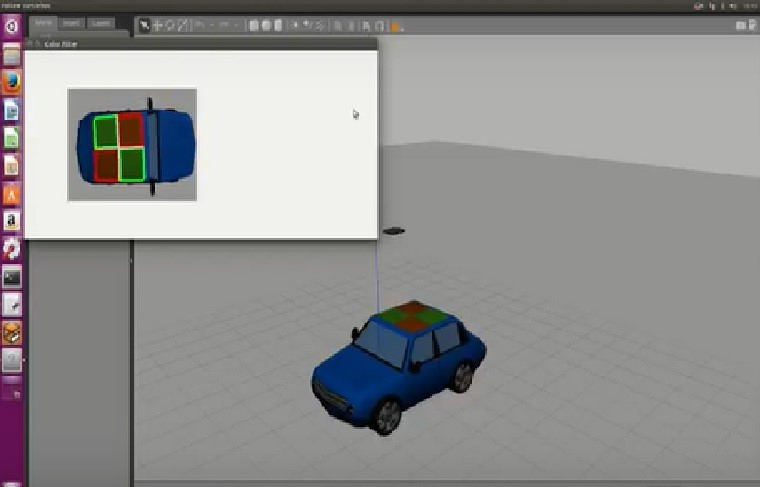
\includegraphics[width=0.4\textwidth]{imgs/TakeOff.jpg}
        \caption{Despegue sobre la baliza del coche.}
	\label{fig:Despegue sobre la baliza del coche}
\end{figure}


\hspace{1cm} Para la realizaci\'on de este experimento con un drone real se sit\'ua la baliza real sobre el suelo y el drone sobre \'esta, y as\'i al despegar ten\'ia un punto sobre el que centrarse. La raz\'on de programar un despegue controlado en vez de en lazo abierto se debe a que el drone real ten\'ia una deriva que le llevaba a desplazarse hacia atr\'as cuando ten\'ia que estar en el sitio. El drone siempre despegaba en esta direcci\'on y hay alrededor de dos segundos en los que no se pueden controlar sus movimientos, por tanto hab\'ia que contar con este desplazamiento. 

\begin{figure}[H]
 \centering
  \subfloat[Despegue vista baliza]{
   \label{f:Vista baliza}
    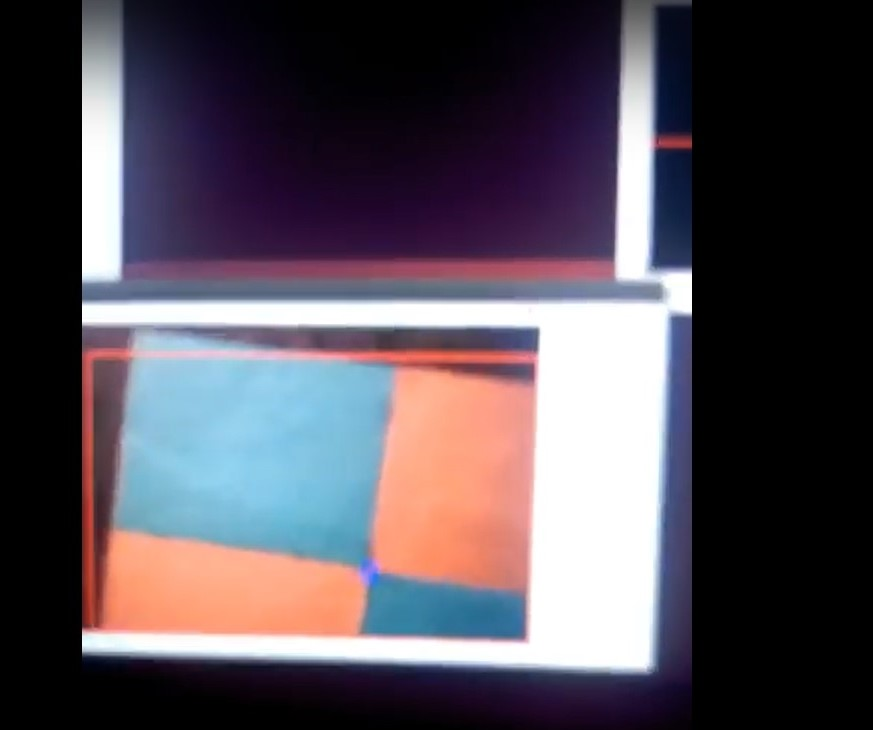
\includegraphics[width=0.36\textwidth]{imgs/takeoff_baliza.jpg}}
  \subfloat[Despegue vista drone]{
   \label{f:Drone}
    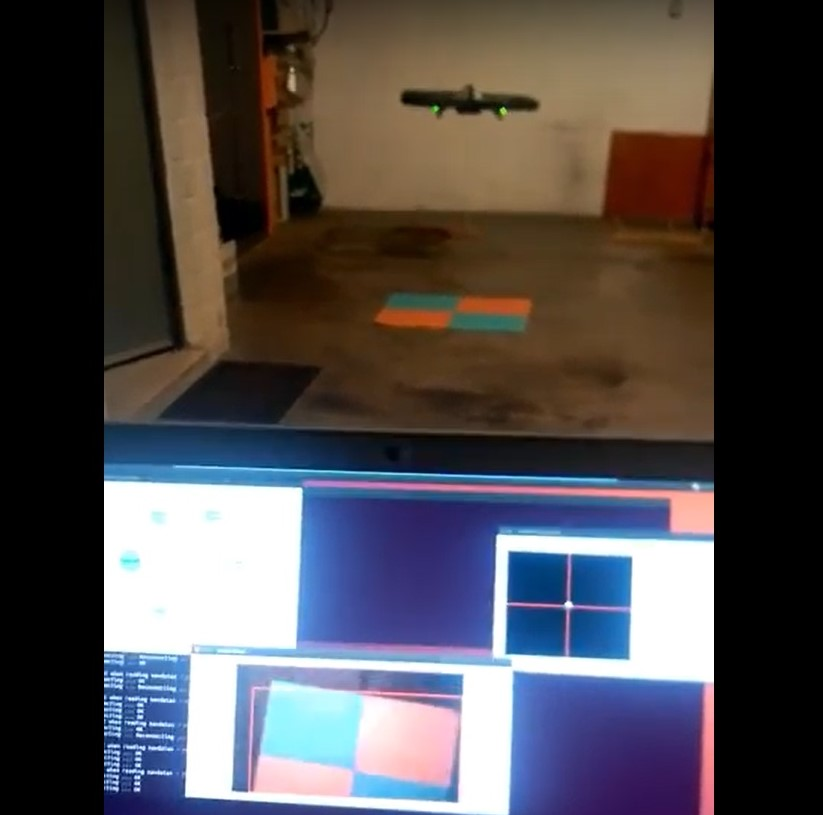
\includegraphics[width=0.36\textwidth]{imgs/takeoff_baliza2.jpg}}
 \caption{Despegue}
 \label{f:Test Despegue}
\end{figure}

Para la realizaci\'on del algoritmo, La duraci\'on del periodo de despegue se controla por tiempo, se ajust\'o en 10 segundos. 
El video de un experimento ilustrativo del despegue del drone real esta disponible en internet. En \'el se puede apreciar un despegue con deriva y la correcci\'on satisfactoria por el software de control desarrollado, de modo que la b\'usqueda de la baliza de destino se inicia mas o menos centrado sobre la baliza de despegue. 
%En el siguiente enlace est\'a el video con el despegue real del drone:\\
\footnote{\url{https://www.youtube.com/watch?v=HVGSlbA1tq4}}

\section{Experimentos de b\'usqueda }
%\hspace{1cm} Para la realizaci\'on de \'esta parte del algoritmo, el drone va movi\'endose en espiral hasta encontrar la baliza, para ya centrarse sobre \'esta. Al principio de los experimentos, el drone se situaba cerca de la baliza para empezar su desplazamiento y que al encontrar la baliza se centrara. Una vez esto funcionaba, se situaba el drone m\'as lejos de \'esta para que en la primera vuelta de la espiral no encontrara ning\'un objeto de inter\'es, pero ya en la segunda vuelta pudiera verlo y se centrara, comprobando de esta forma que las espirales se realizaban de forma correcta. En los primeros experimentos el control, pues solo ten\'ia componente proporcional y el momento que pasaba de no detectar nada a encontrar una posible baliza los movimientos eran muy bruscos, arreglando esto con el control PID. 

\hspace{1cm} Para la realizaci\'on de esta parte del algoritmo, el drone va movi\'endose en espiral hasta encontrar la baliza, para ya centrarse sobre \'esta. Se han realizado diversos experimentos. Por una parte escenarios donde el punto de despegue y el de aterrizaje se sit\'uan muy cerca, por tanto tiene que despegar, detectar la otra baliza y centrarse sobre esta. Por otro lado, escenarios situando lejos la baliza de despegue y de aterrizaje, observando as\'i que el drone ampliaba su recorrido en cada vuelta de espiral que daba. Adem\'as, en ambas pruebas se han controlado las velocidades del drone para evitar movimientos bruscos. 


\begin{figure}[H]
 \centering
    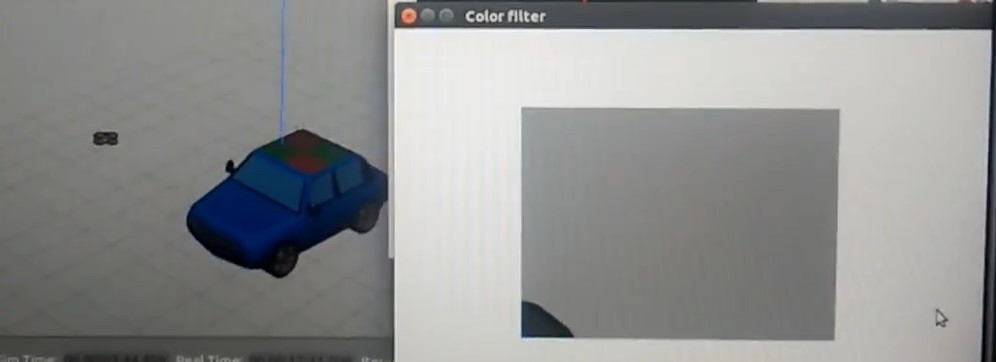
\includegraphics[width=0.33\textwidth]{imgs/busqueda1.jpg}
    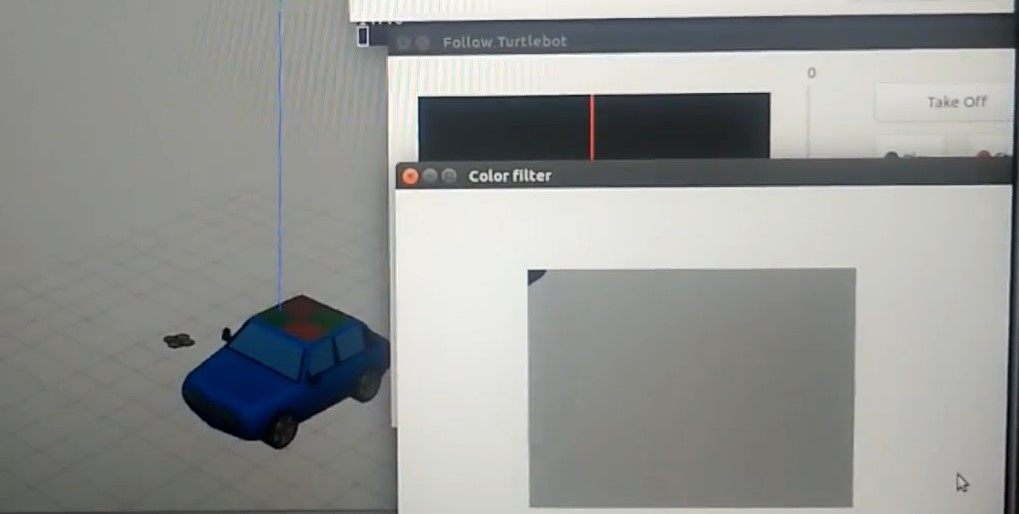
\includegraphics[width=0.32\textwidth]{imgs/busqueda3.jpg}
    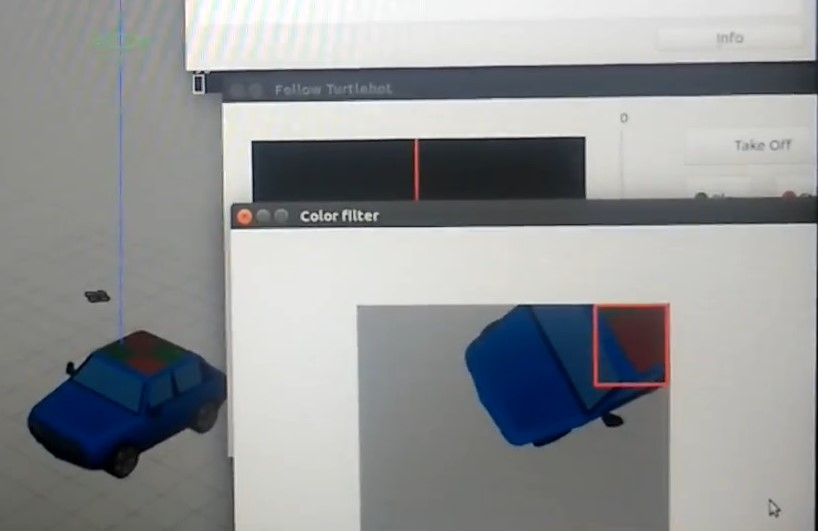
\includegraphics[width=0.29\textwidth]{imgs/busqueda5.jpg}\\
    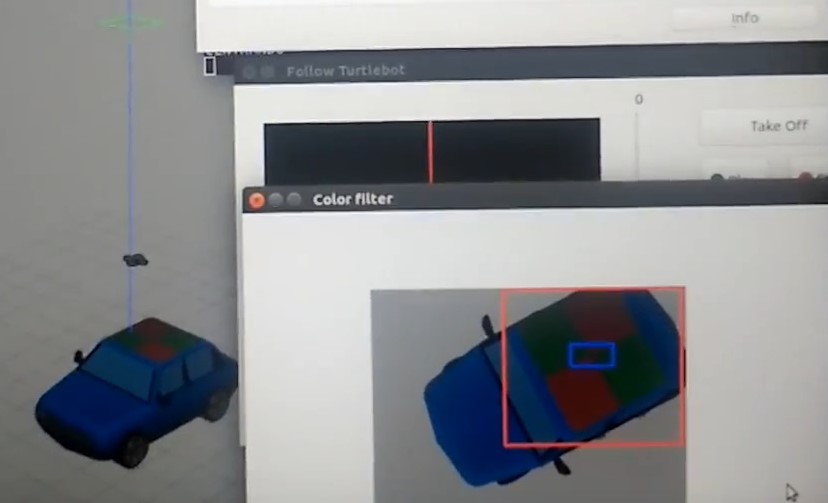
\includegraphics[width=0.39\textwidth]{imgs/busqueda6.jpg}
    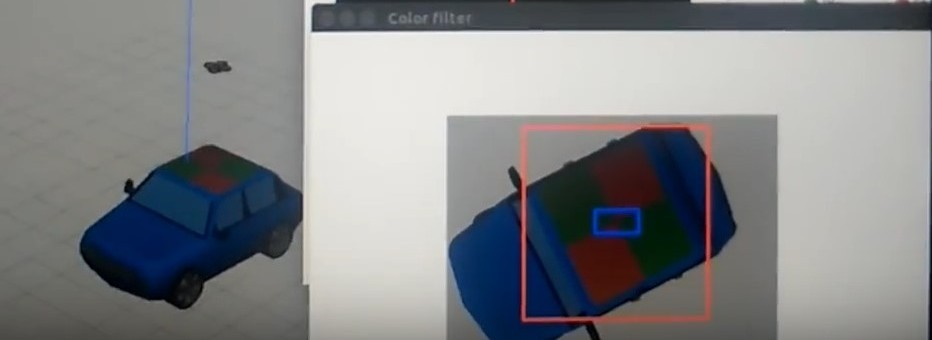
\includegraphics[width=0.4\textwidth]{imgs/busqueda7.jpg}
 \caption{B\'usqueda en espiral en escenario simulado}
 \label{f:Busqueda sobre el simulador}
\end{figure}


%\hspace{1cm} Para las pruebas con del drone real, primero se prob\'o solo que el algoritmo de b\'usqueda era correcto, y que el drone realizaba espirales de forma correcta. Pero despu\'es, al realizar las pruebas finales en espacios m\'as pequeños se modific\'o el algoritmo de b\'usqueda, haciendo que el drone se moviera haciendo cuadrados para tener un mayor control sobre \'este. 

\hspace{1cm} Para las pruebas del drone real, se han realizado tambi\'en dos pruebas principales. Por un lado se han realizado varios tests detectando que el drone hac\'ia espirales de forma correcta, ampliando la trayectoria de forma continua. Por otro lado que al detectar la baliza no realizara movimientos bruscos para centrarse sobre esta. Destacar que para la realizaci\'on de pruebas en lugares poco espaciosos se program\'o otra variante del algoritmo de b\'usqueda, pasando de hacer espirales a hacer cuadrados, para tener un movimiento m\'as controlado del drone. 


\begin{figure}[H]
 \centering
    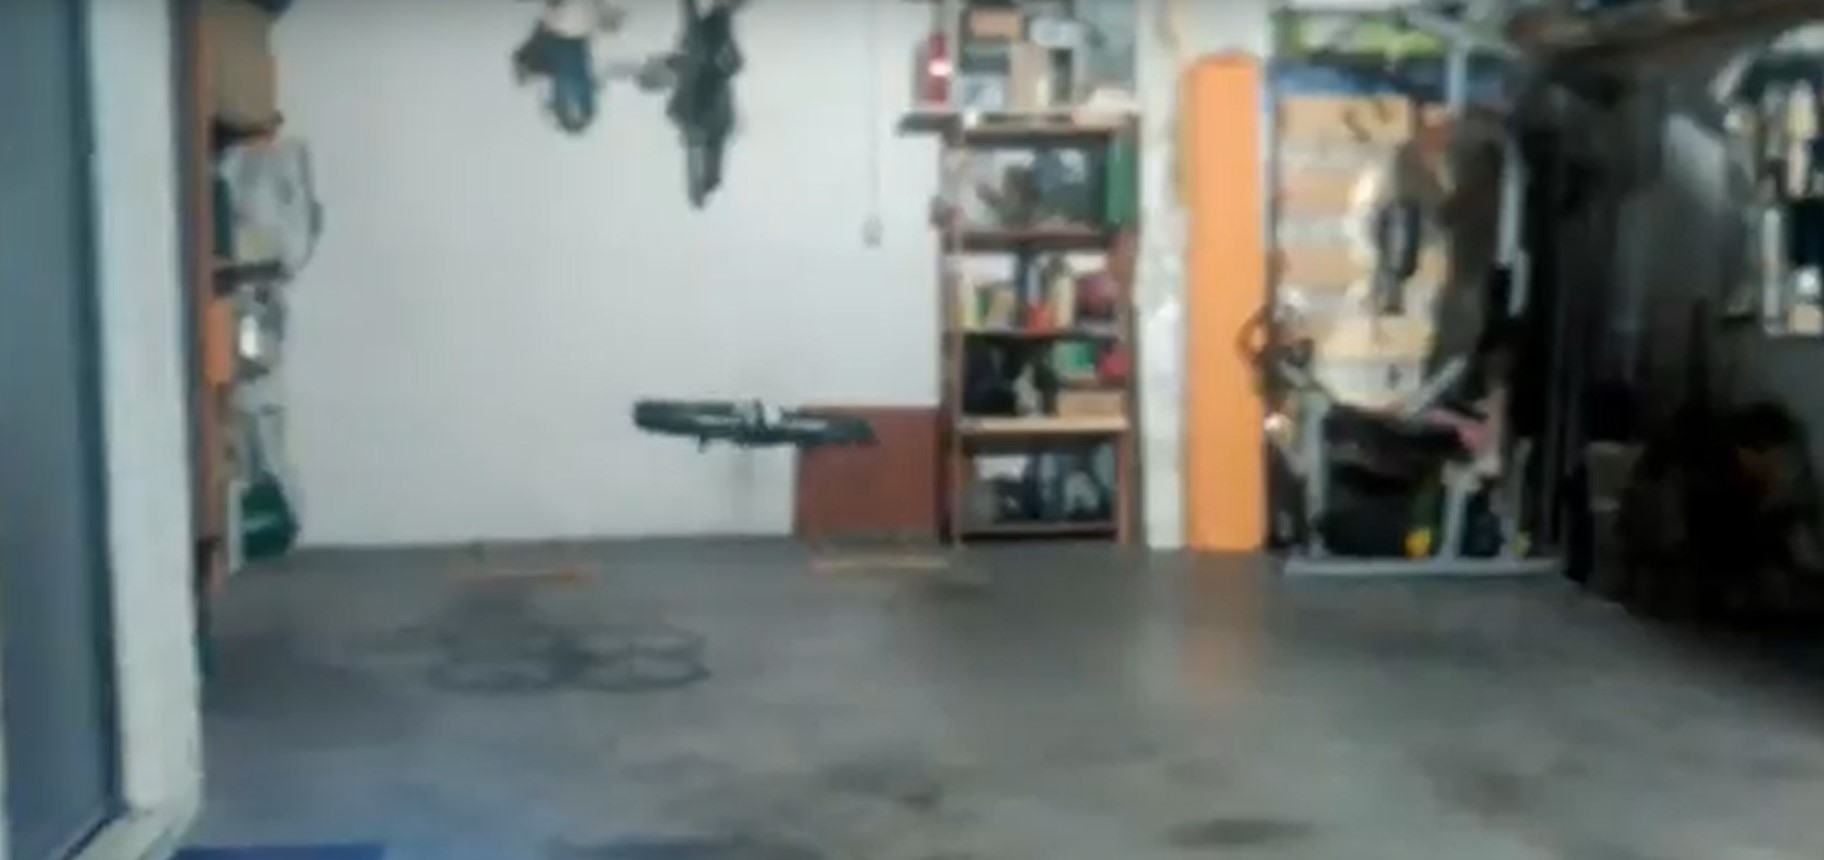
\includegraphics[width=0.33\textwidth]{imgs/busqueda_real1.jpg}
    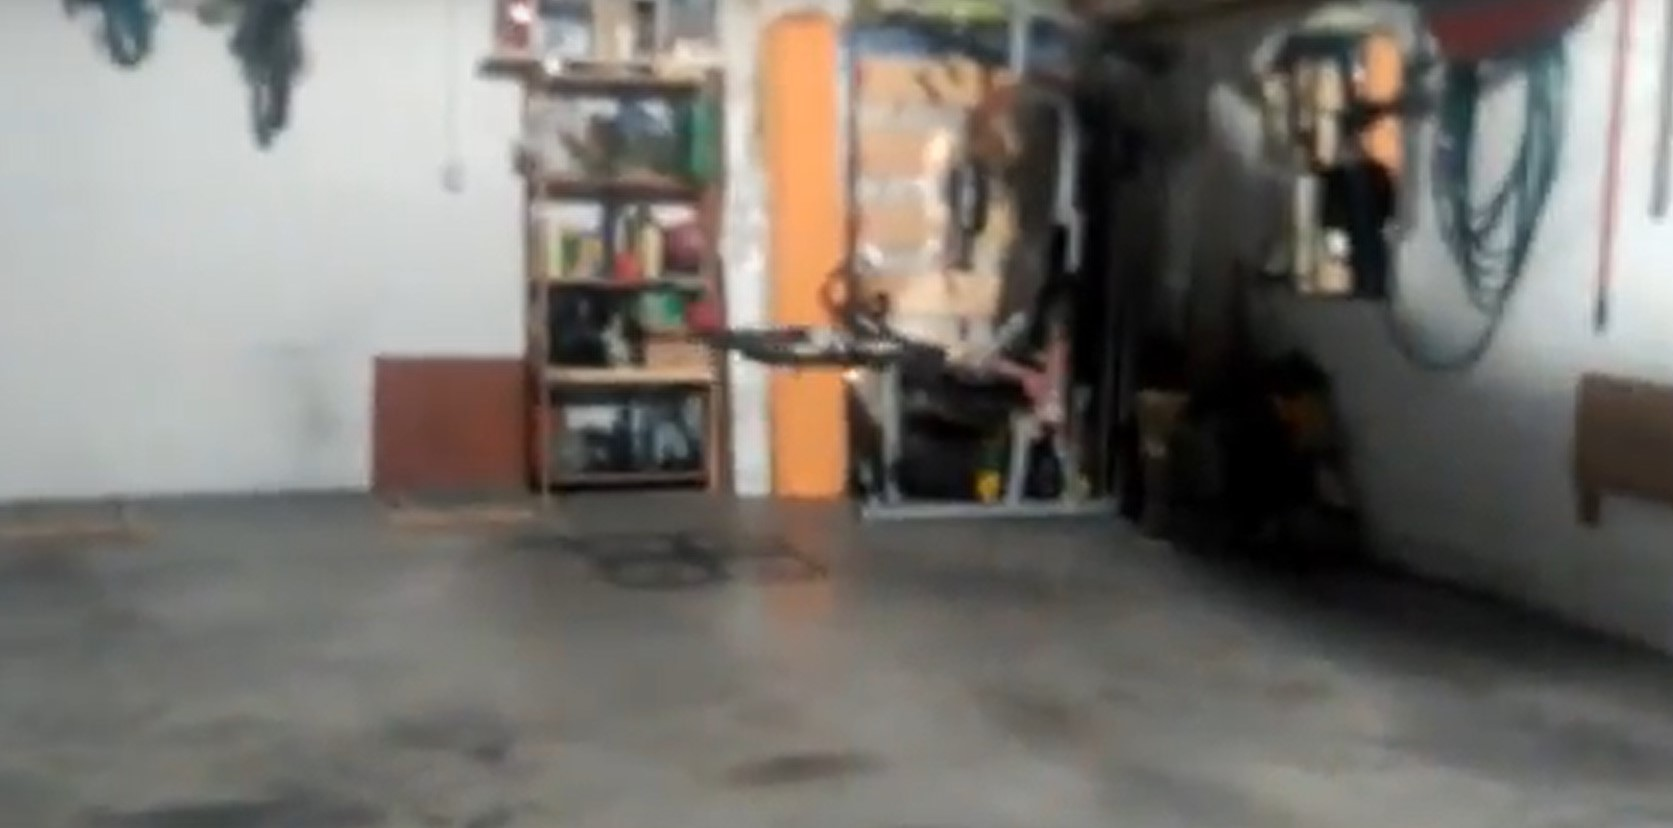
\includegraphics[width=0.32\textwidth]{imgs/busqueda_real3.jpg}
    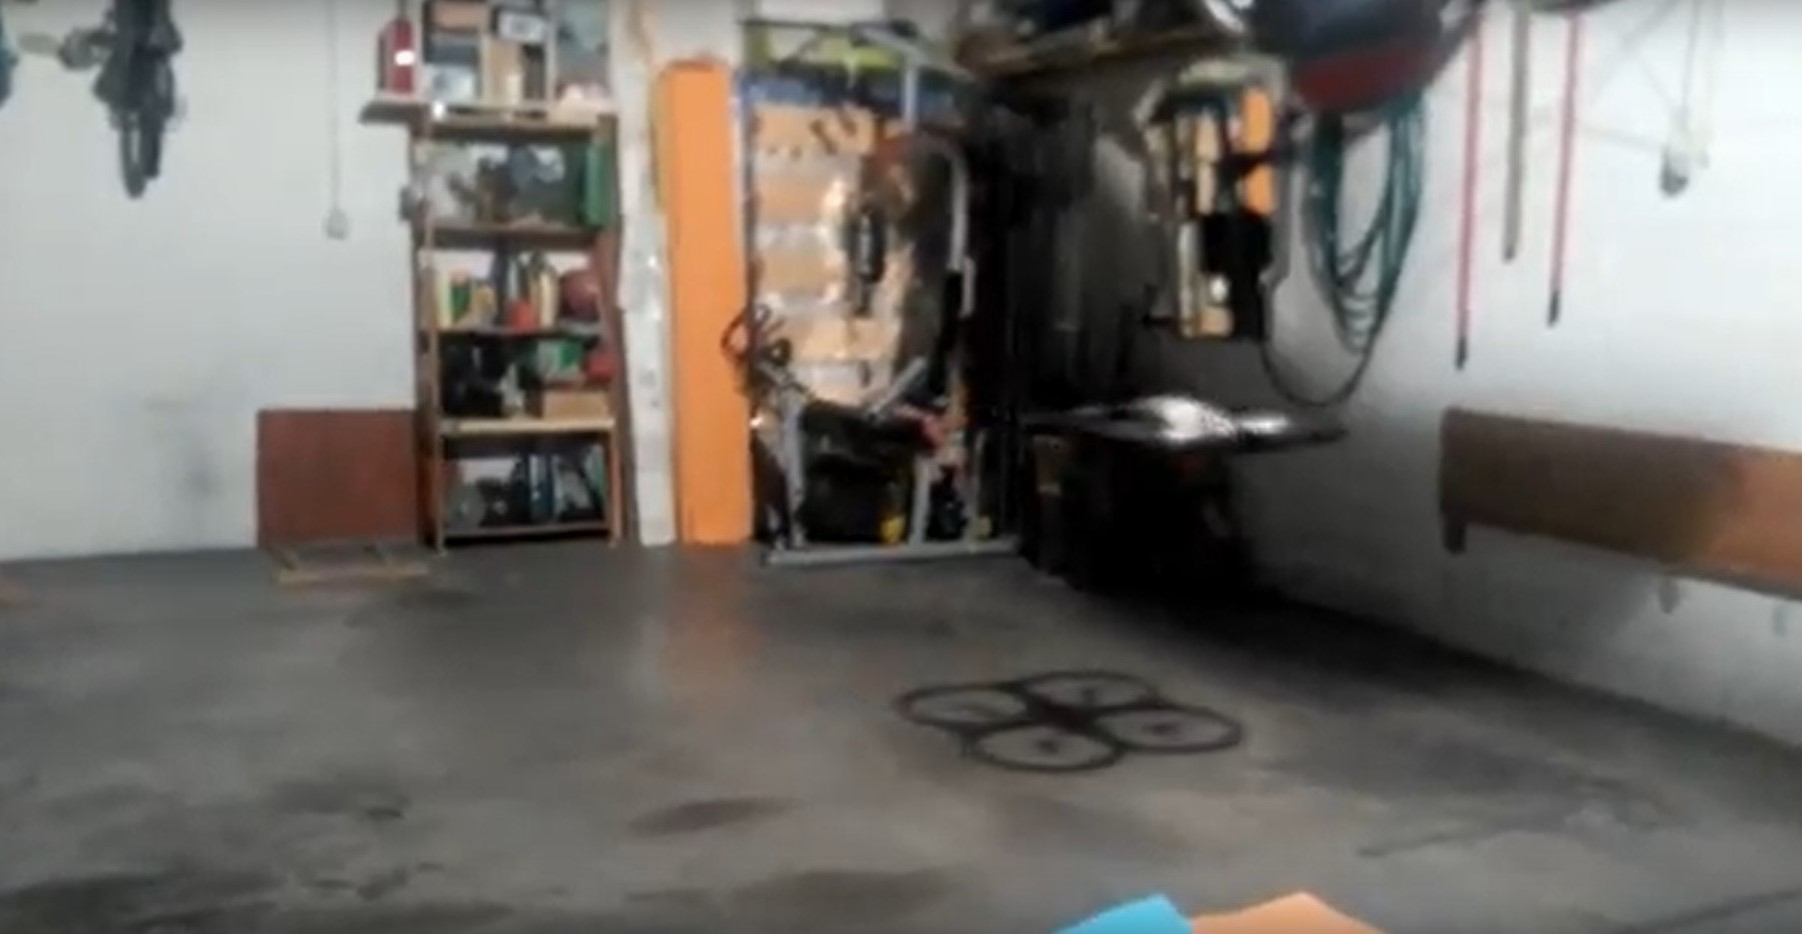
\includegraphics[width=0.30\textwidth]{imgs/busqueda_real5.jpg}\\
    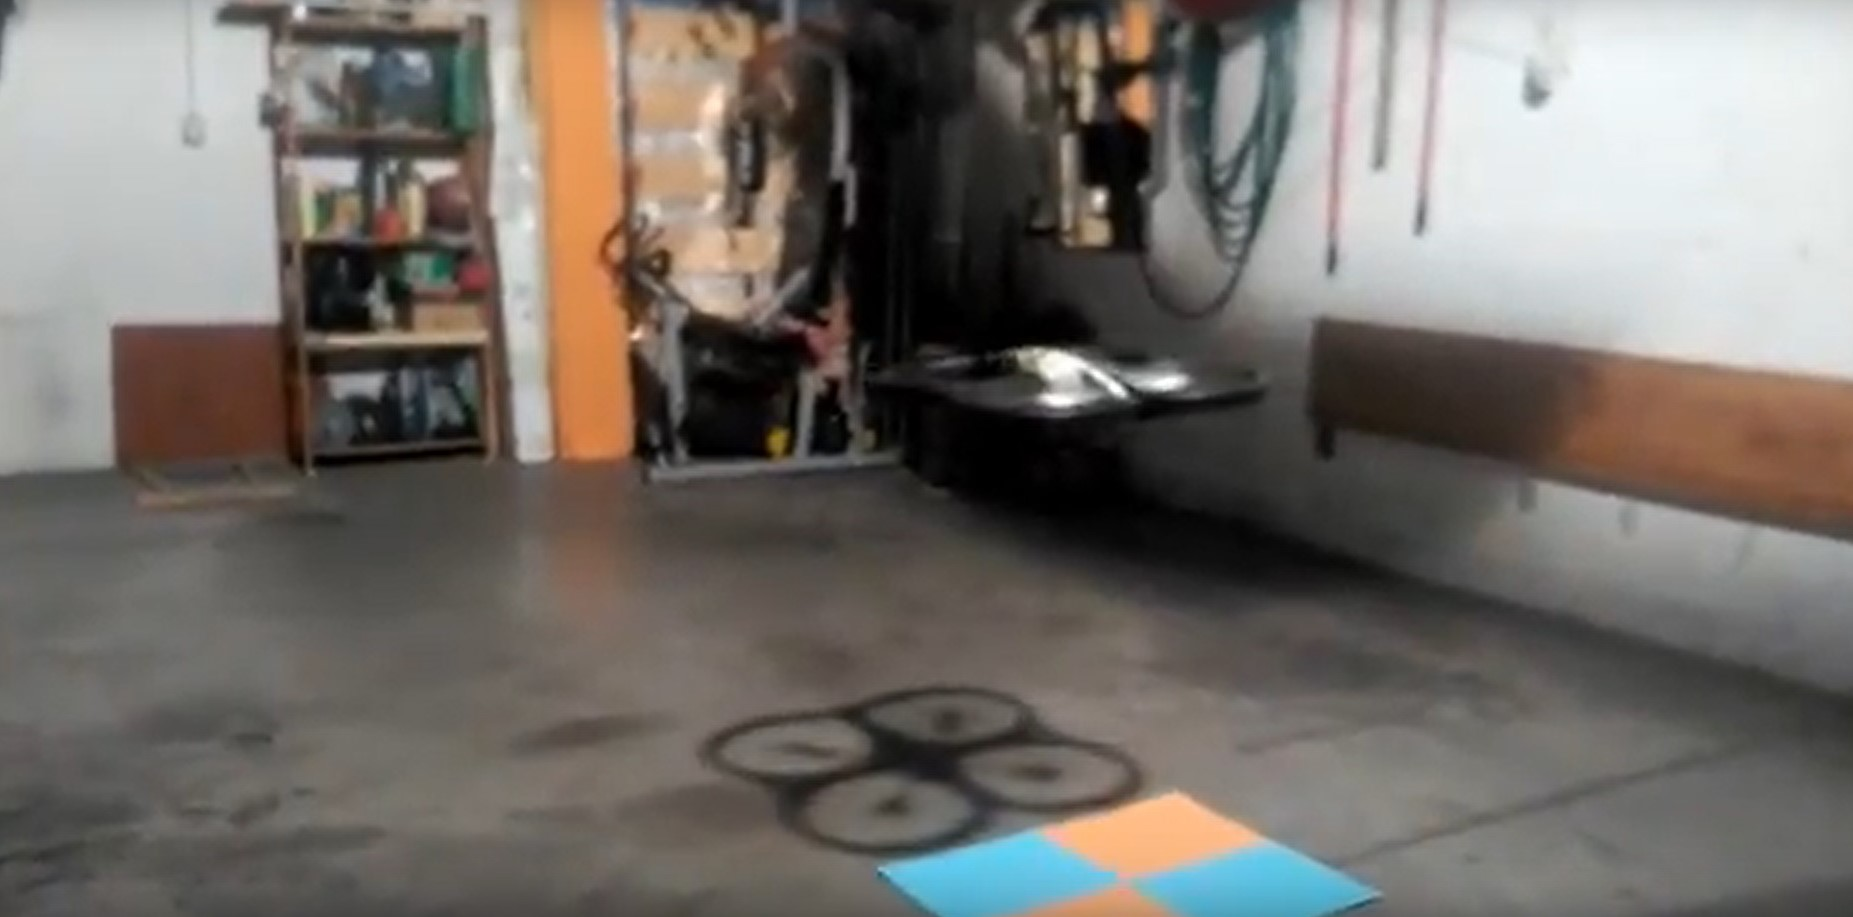
\includegraphics[width=0.4\textwidth]{imgs/busqueda_real6.jpg}
    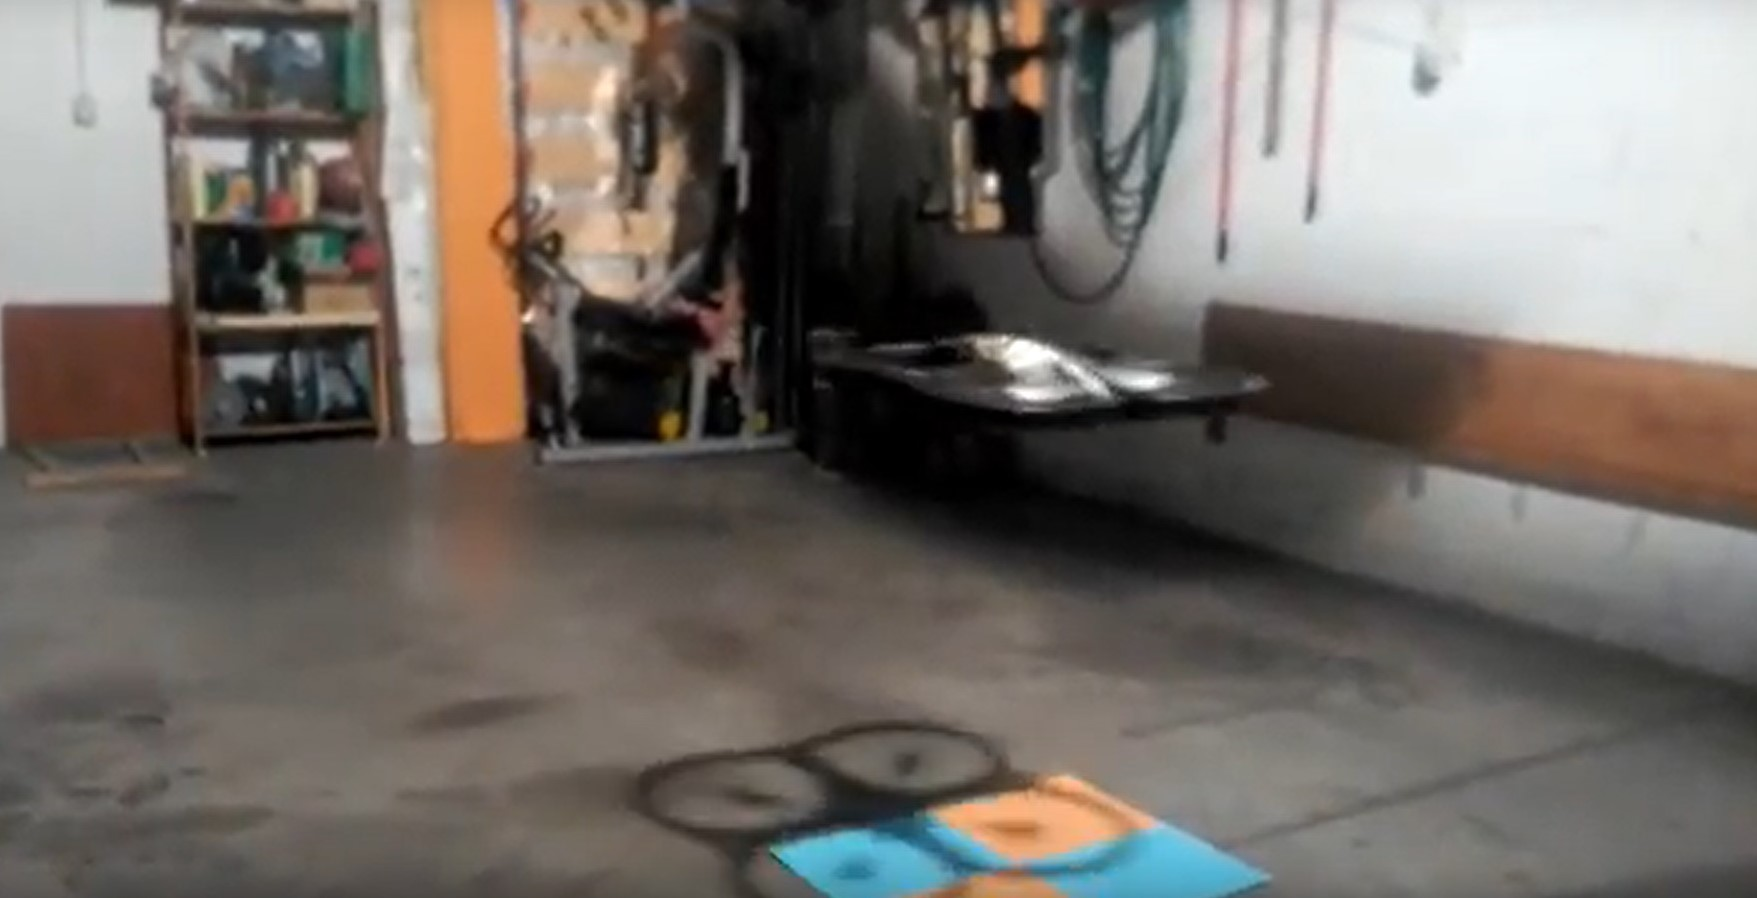
\includegraphics[width=0.38\textwidth]{imgs/busqueda_real7.jpg}
 \caption{B\'usqueda en el escenario real}
 \label{f:Busqueda con el drone real}
\end{figure}


\section{Experimentos de aterrizaje}

\hspace{1cm} En los experimentos de esta parte, se trat\'o de verificar que el drone se centrara sobre la baliza sin realizar movimientos bruscos, una vez que el drone detectaba que estaba pr\'acticamente centrado sobre la baliza, comenzaba a descender, y una vez detectaba que estaba lo suficientemente cerca enviaba la orden de parar.% En estos experimentos la parte de percepci\'on se basan en controlar el centro de la baliza y el \'area, para tener una aproximaci\'on de la distancia que hay a \'esta. 

\begin{figure}[H]
 \centering
    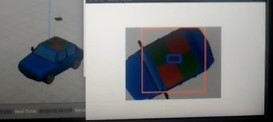
\includegraphics[width=0.45\textwidth]{imgs/landing1_1.jpg}
    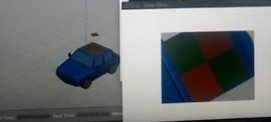
\includegraphics[width=0.45\textwidth]{imgs/landing2_1.jpg}
    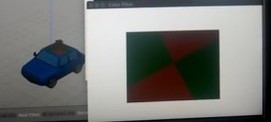
\includegraphics[width=0.45\textwidth]{imgs/landing3_1.jpg}
    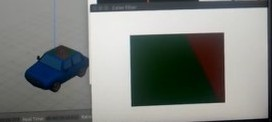
\includegraphics[width=0.45\textwidth]{imgs/landing4_1.jpg}
 \caption{Aterrizaje}
 \label{f:Aterrizaje sobre el simulador}
\end{figure}


\hspace{1cm} En la primera prueba, cuando el drone estaba en el aire se pon\'ia delante de la baliza de un color y al detectarla apagaba motores directamente. En la segunda prueba, cuando el drone estaba en el aire, en lugar de mostrar la baliza a la c\'amara frontal se le mostro a la c\'amara de abajo, probando as\'i el funcionamiento de la camara y que detectaba la baliza que se iba a utilizar. En la tercera prueba, mientras realizaba el algoritmo de b\'usqueda, una vez detectara la baliza aterrizara. En esta prueba los resultados eran buenos, ya que se consegu\'ia que aterrizara, pero por la velocidad que ten\'ia el drone y debido a la inercia, no aterrizaba en el sitio exacto sino que segu\'ia en la misma direcci\'on que ten\'ia anteriormente hasta que se posaba en el suelo y ya se deten\'ia, por lo tanto aterrizaba en las proximidades, pero relativamente tras esto y al añadir el control para centrarse sobre \'esta, se solucion\'o el problema y se consigui\'o que el drone aterrizara verticalmente sobre la baliza. 

\begin{figure}[H]
 \centering
    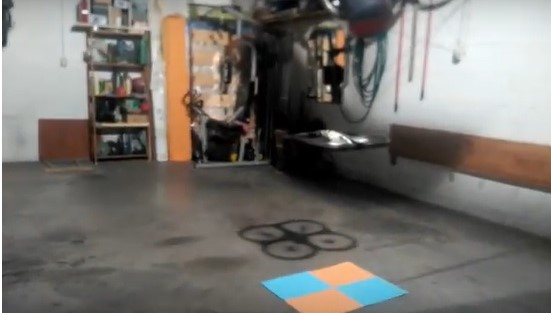
\includegraphics[width=0.30\textwidth]{imgs/aterrizaje_real1.jpg}
    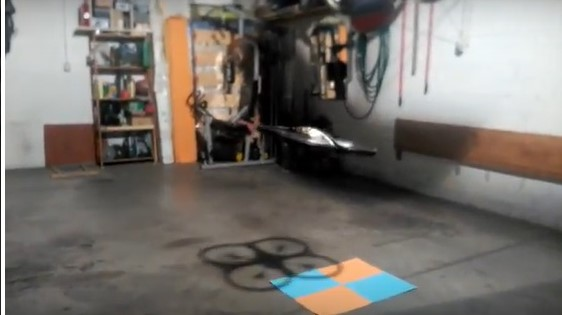
\includegraphics[width=0.30\textwidth]{imgs/aterrizaje_real2.jpg}
    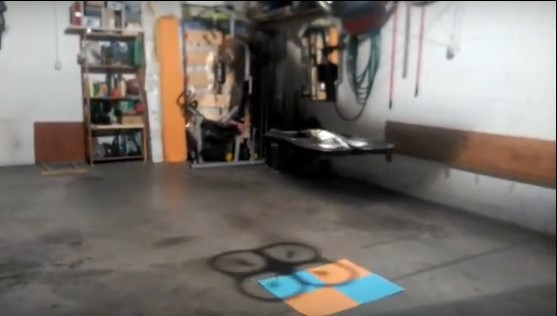
\includegraphics[width=0.30\textwidth]{imgs/aterrizaje_real3.jpg}\\
    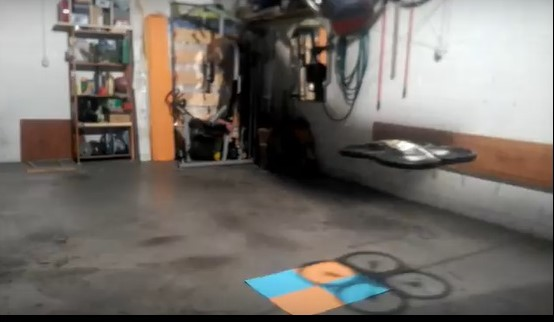
\includegraphics[width=0.30\textwidth]{imgs/aterrizaje_real4.jpg}
    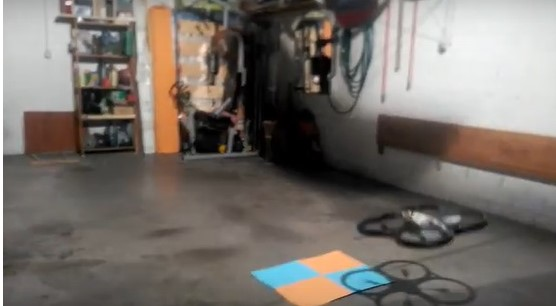
\includegraphics[width=0.30\textwidth]{imgs/aterrizaje_real5.jpg}
    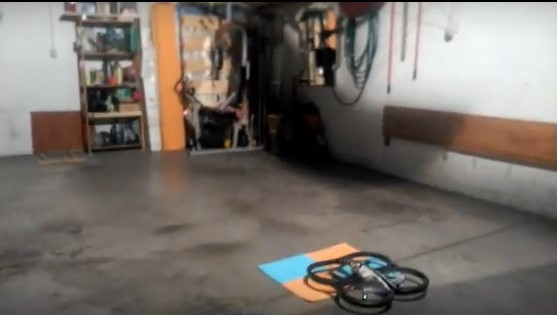
\includegraphics[width=0.30\textwidth]{imgs/aterrizaje_real6.jpg}
 \caption{Aterrizaje}
 \label{f:Aterrizaje con el drone real.}
\end{figure}


\section{Ejecuci\'on t\'ipica del algoritmo completo}\label{sec.algoritmocompleto}
\hspace{1cm} Una vez validada cada una de las partes del algoritmo, tanto perceptivas como de control, se realizaron varios experimentos con todo el sistema integrado.

\hspace{1cm} Este experimento se realiz\'o para comprobar que todo lo que se hab\'ia programado por partes funcionaba tambi\'en si se probaba el algoritmo completo. Las pruebas salieron correctamente.

\hspace{1cm} Sobre el simulador se prob\'o a poner el drone sobre la baliza, que despegaba y se situaba en el centro de \'esta. Una vez pasaron 10 segundos y el drone continuaba en el centro, se hizo que \'este se alejara y perdiera la referencia de la baliza, y comenzara su algoritmo de b\'usqueda. Una vez realizaba las espirales, en el momento que detectaba los colores de la baliza de destino se centraba sobre estos, y una vez estaba aproximadamente centrado, comenzaba a descender hasta que detectaba que estaba a una altura suficiente y se le pod\'ia mandar la orden de aterrizar, pos\'andose as\'i sobre la baliza. 

En la figura \ref{f:Algoritmo completo sobre el simulador} se muestra la secuencia de im\'agenes con el despegue y el drone alej\'andose de la baliza. Las im\'agenes de la b\'usqueda y el aterrizaje est\'an en las figuras \ref{f:Busqueda sobre el simulador} y \ref{f:Aterrizaje sobre el simulador}. La referencia con el v\'ideo es \footnote{\url{https://www.youtube.com/watch?v=g9ZGJhRWTiY}}

\begin{figure}[H]
 \centering
  \subfloat[Despegue]{
   \label{f:Despegue}
    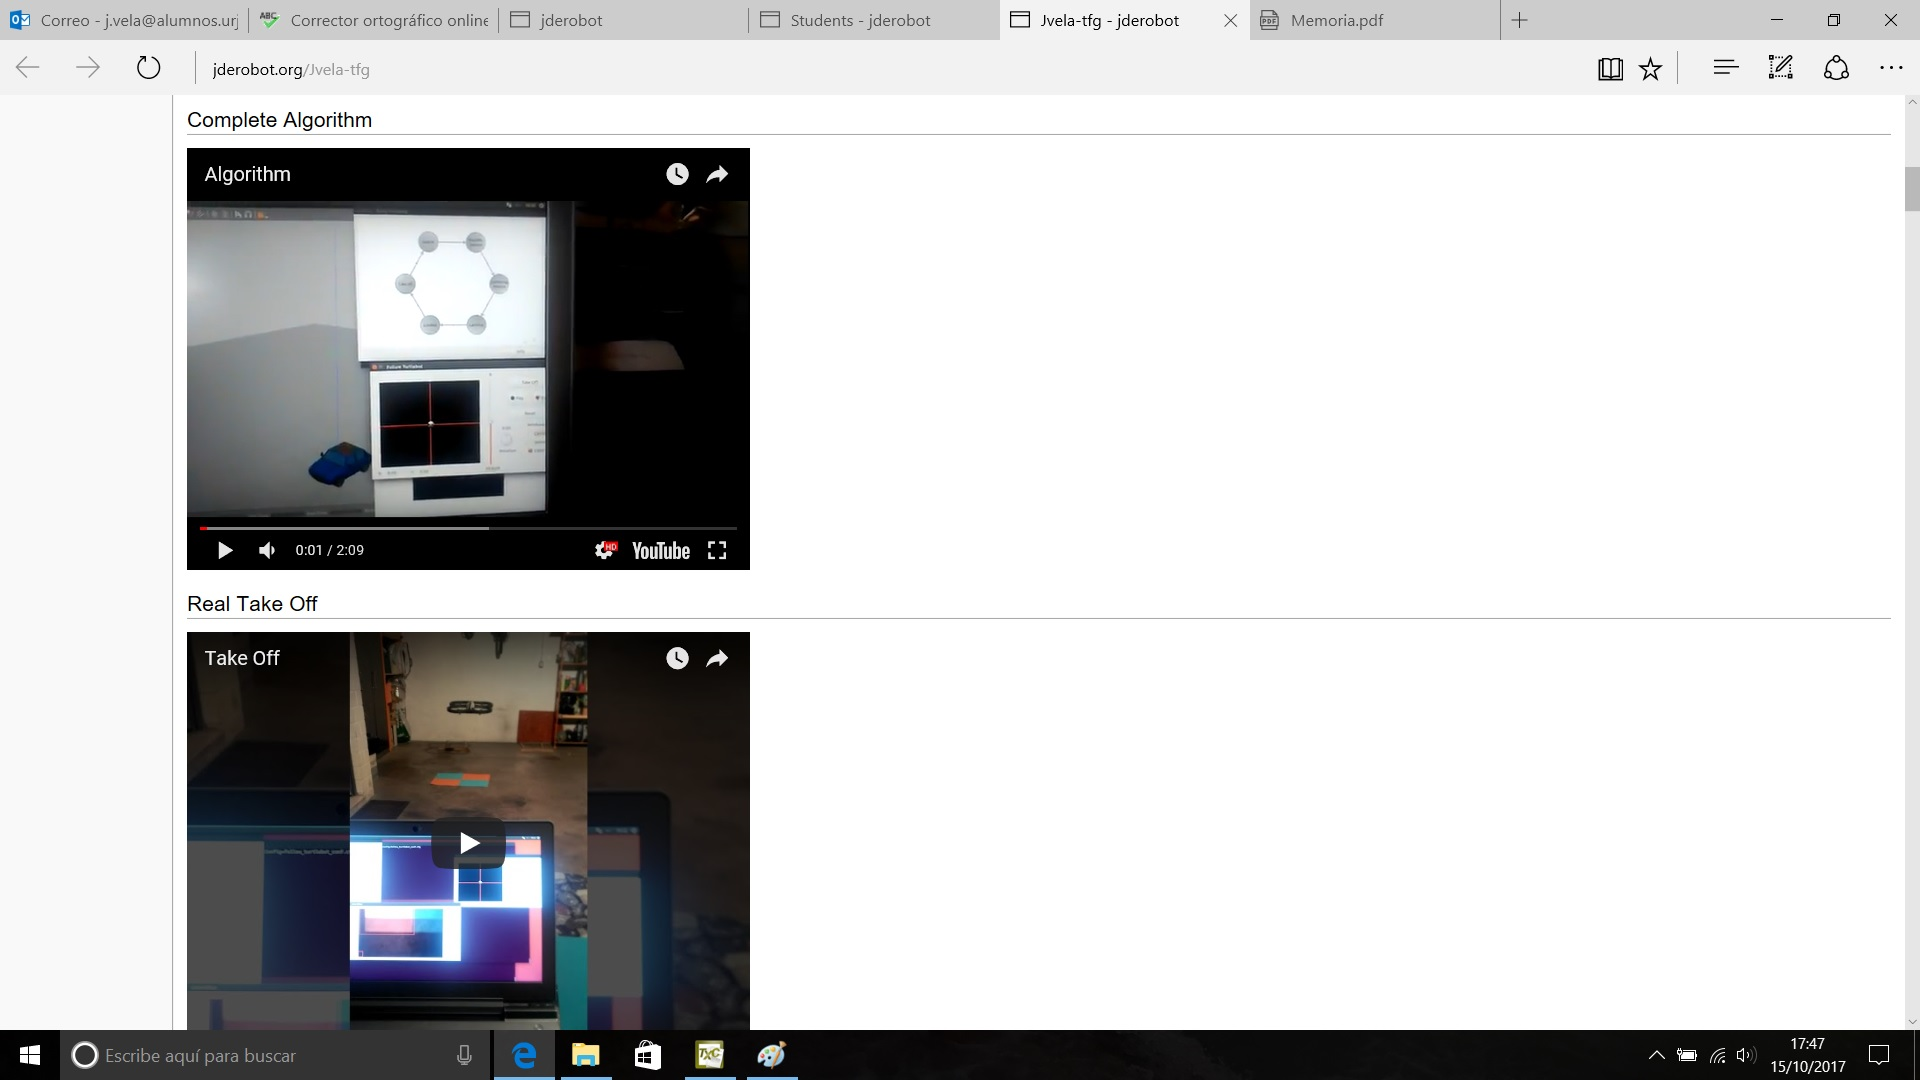
\includegraphics[width=0.25\textwidth]{imgs/total1.jpg}}
  \subfloat[Despegue]{
   \label{f:Despegue}
    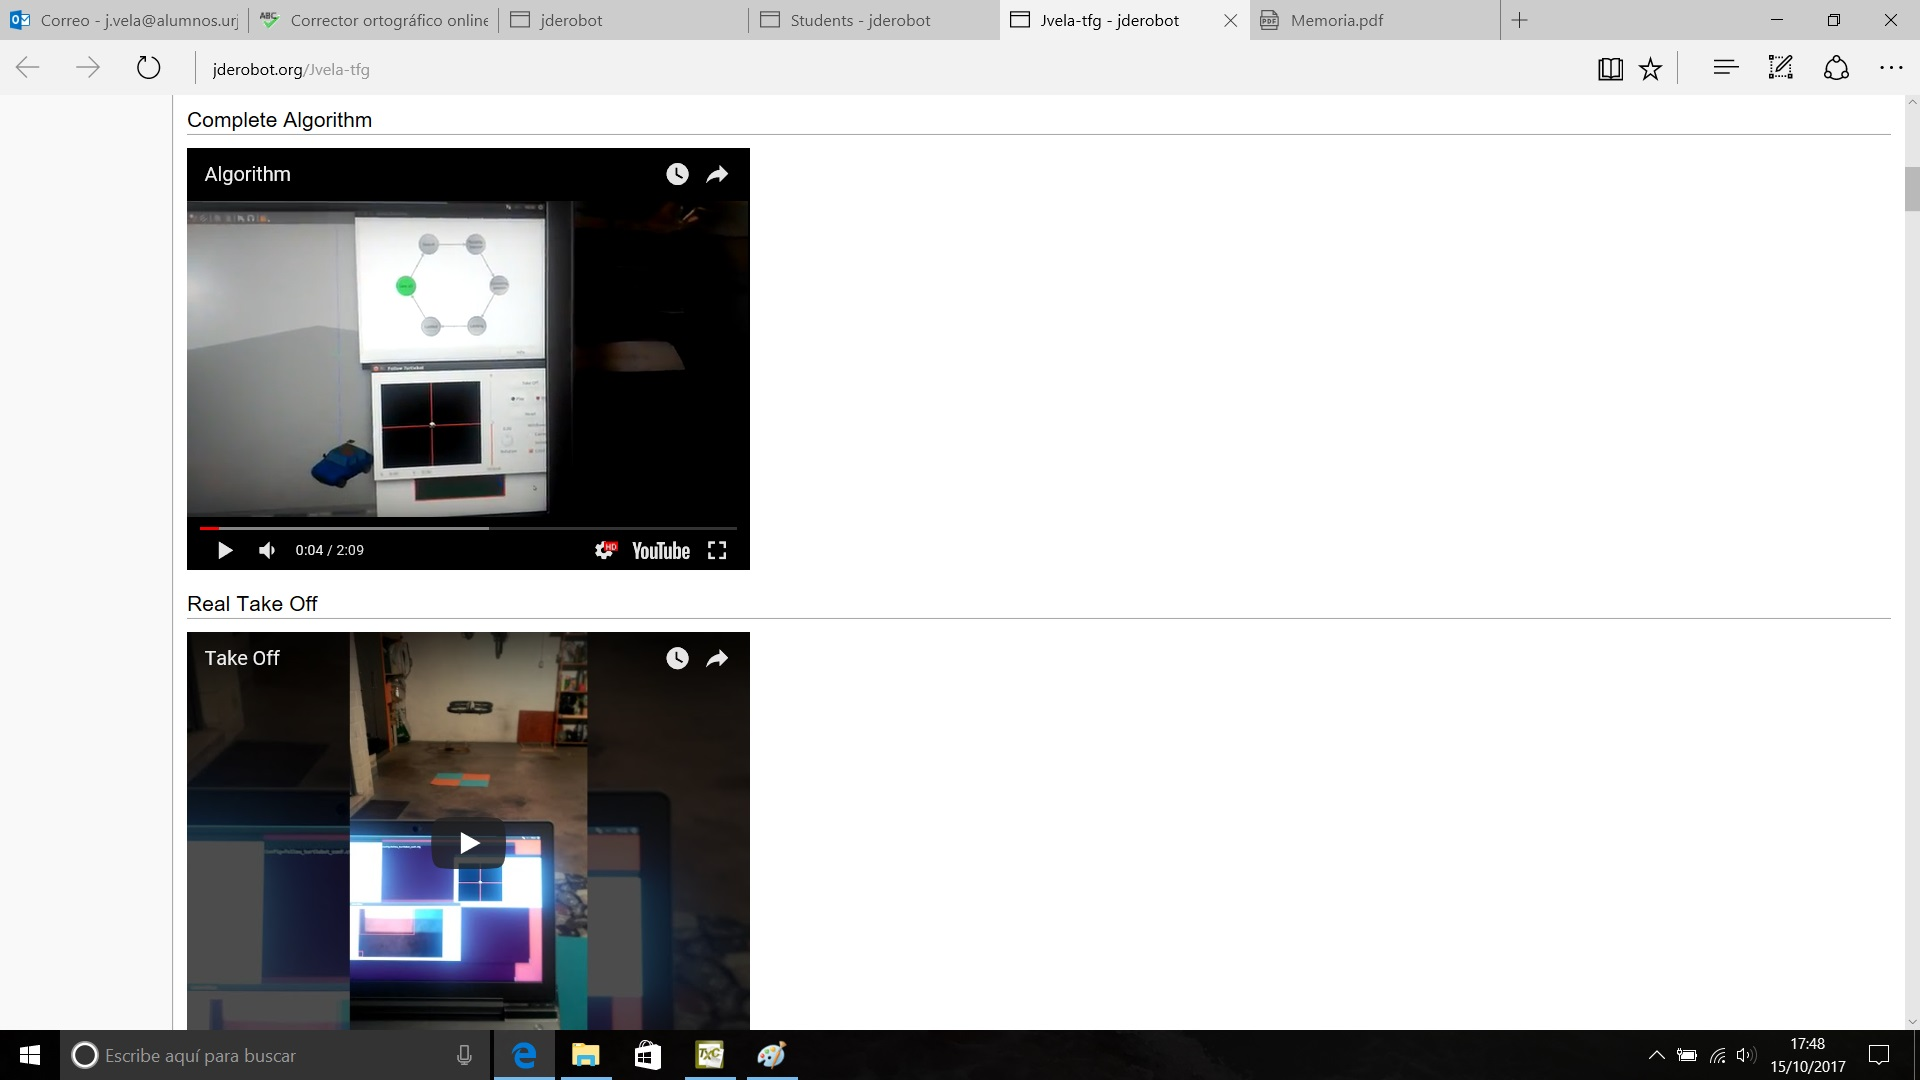
\includegraphics[width=0.25\textwidth]{imgs/total2.jpg}}
	\subfloat[Despegue]{
   \label{f:Despegue}
    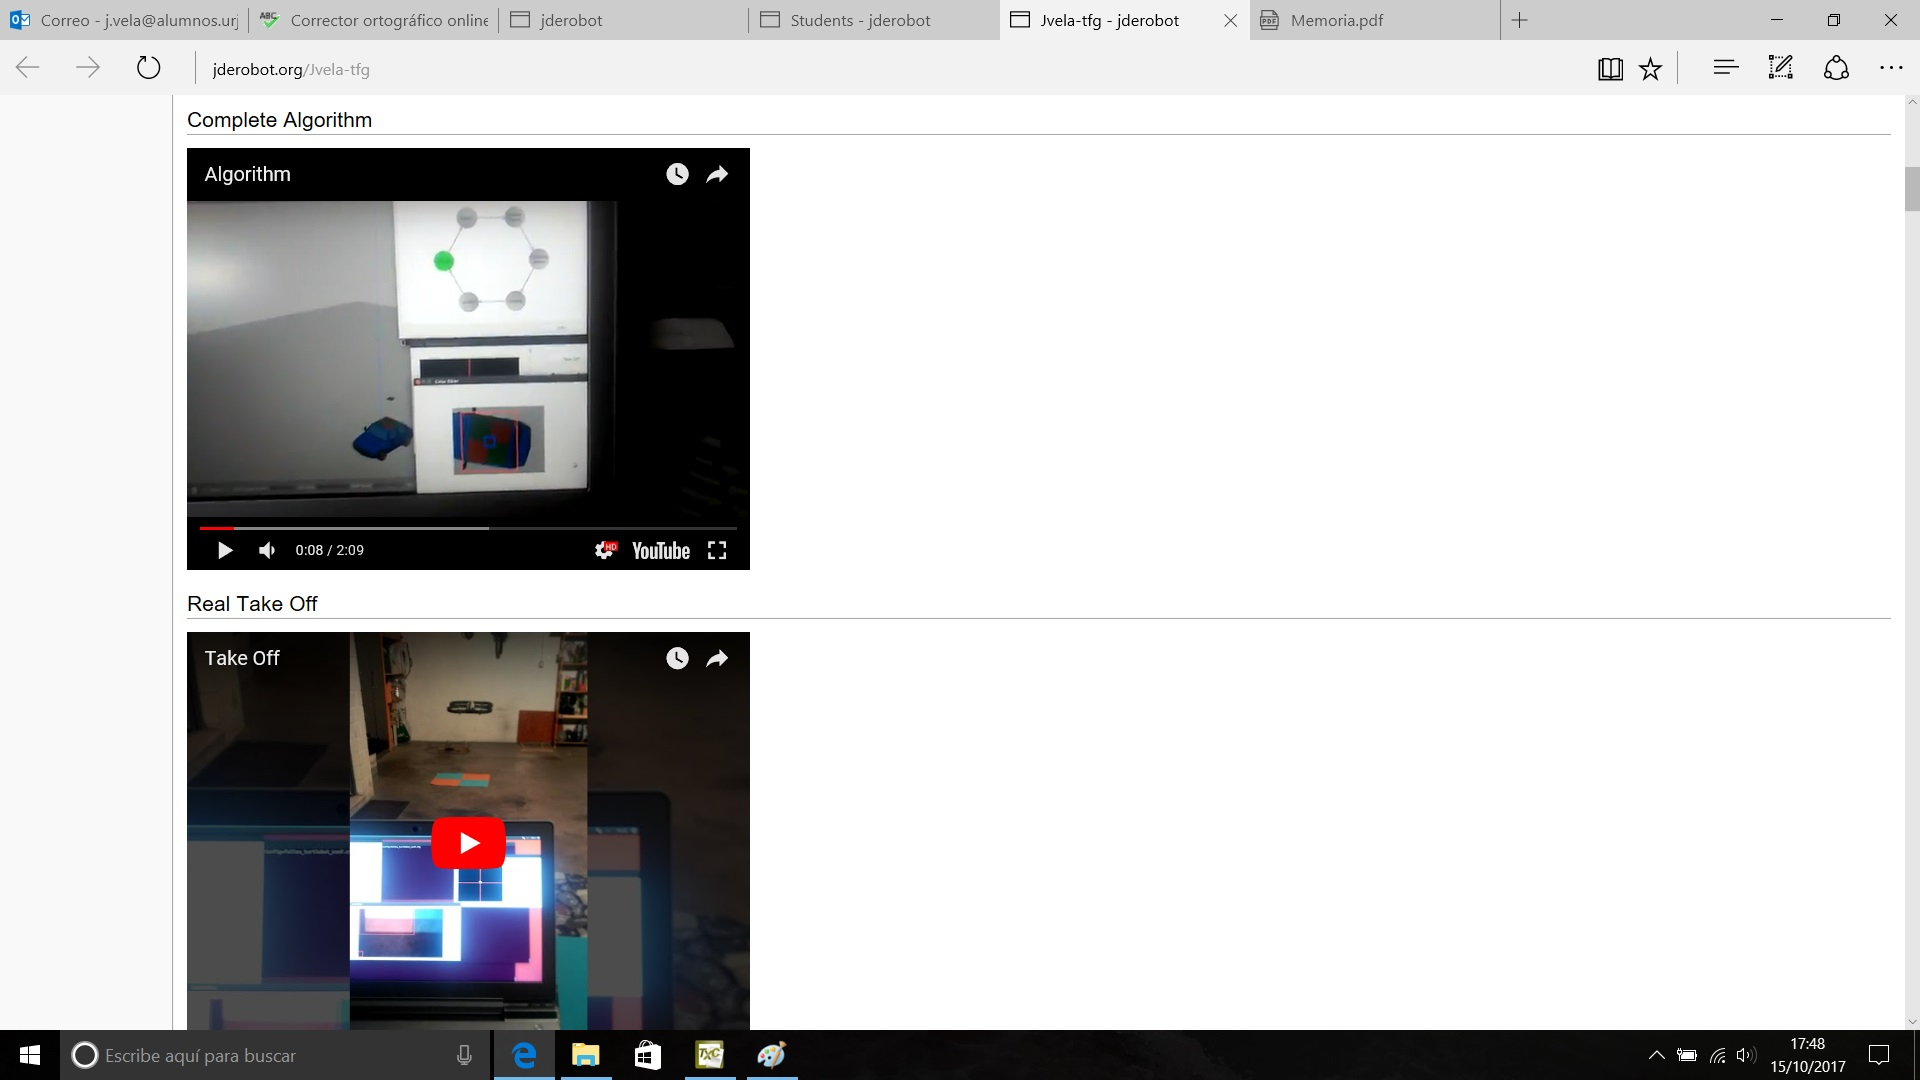
\includegraphics[width=0.25\textwidth]{imgs/total3.jpg}}
	\subfloat[Despegue]{
   \label{f:Despegue}
    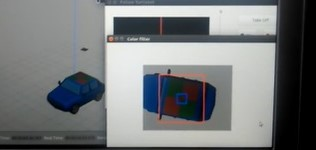
\includegraphics[width=0.25\textwidth]{imgs/total4.jpg}}\\
	\subfloat[Alejandose de la baliza]{
   \label{f:Alejandose de la baliza}
    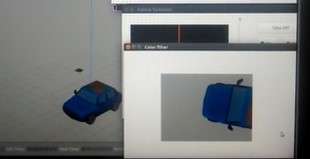
\includegraphics[width=0.25\textwidth]{imgs/total5.jpg}}
	%\subfloat[Busqueda]{
  % \label{f:Busqueda}
  %  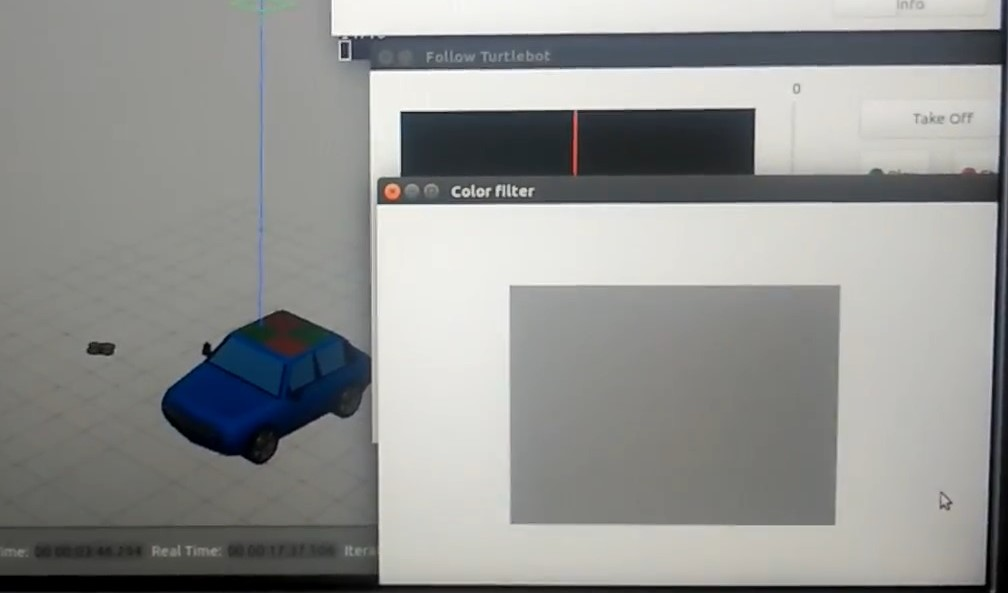
\includegraphics[width=0.25\textwidth]{imgs/busqueda2.jpg}}
	%\subfloat[Busqueda]{
  % \label{f:Busqueda}
  %  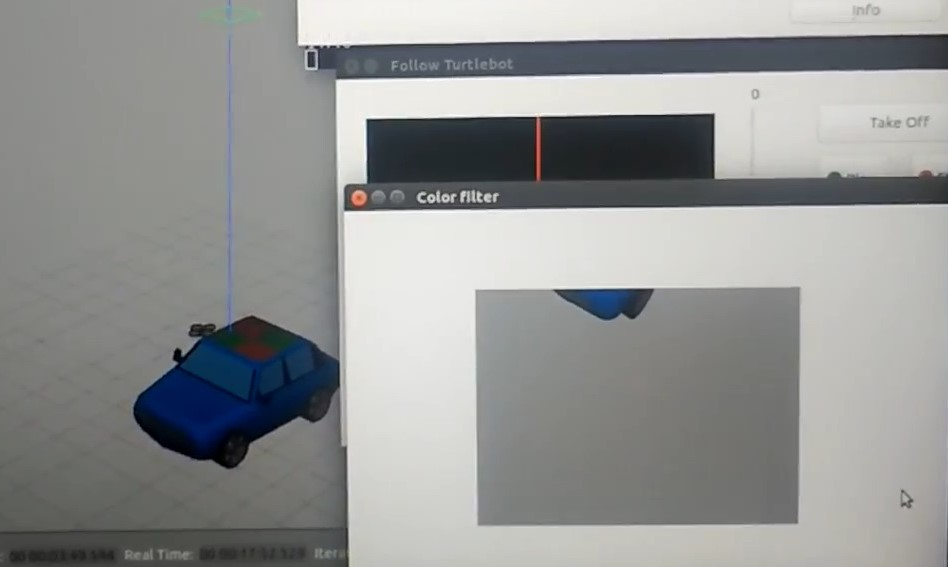
\includegraphics[width=0.25\textwidth]{imgs/busqueda4.jpg}}
	%\subfloat[Busqueda]{
  % \label{f:Busqueda}
  %  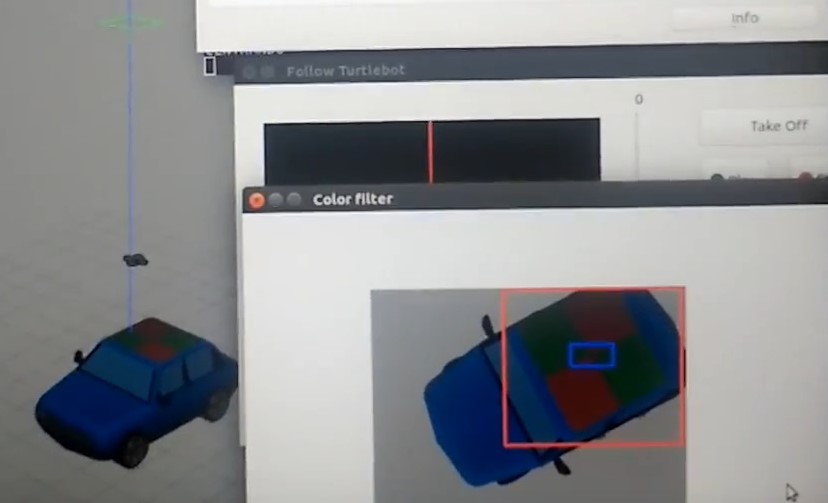
\includegraphics[width=0.25\textwidth]{imgs/busqueda6.jpg}} \\
	%	  \subfloat[Aterrizaje]{
  % \label{f:Aterrizaje}
  %  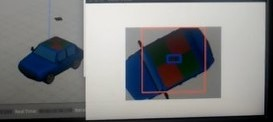
\includegraphics[width=0.25\textwidth]{imgs/landing1.jpg}}
  %\subfloat[Aterrizaje]{
  % \label{f:Aterrizaje}
  %  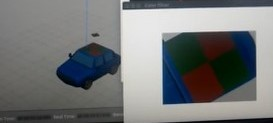
\includegraphics[width=0.30\textwidth]{imgs/landing2.jpg}}
	%\subfloat[Aterrizaje]{
  % \label{f:Aterrizaje}
  %  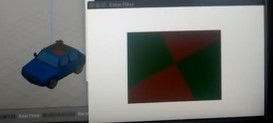
\includegraphics[width=0.25\textwidth]{imgs/landing3.jpg}}
	%\subfloat[Aterrizaje]{
  % \label{f:Aterrizaje}
  %  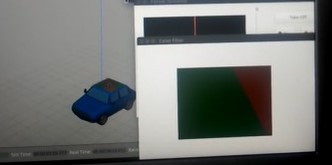
\includegraphics[width=0.25\textwidth]{imgs/landing4.jpg}}
 \caption{Algoritmo completo de navegaci\'on en escenario simulado. }
 \label{f:Algoritmo completo sobre el simulador}
\end{figure}


\hspace{1cm} Para las prueba con el drone real se colocaron dos puntos de referencia. Una baliza sobre la que situarse al despegar. De esta forma al comenzar el algoritmo, cuando detectaba esta baliza se centraba sobre \'esta, y una vez pasaron 10 segundos comenzaba el algoritmo de b\'usqueda. En este punto, el drone se mueve en forma de espiral. En las siguientes im\'agenes puede verse c\'omo en una primera vuelta de la espiral el drone no llega a ver la baliza de destino. Sin embargo, en la segunda vuelta de la espiral ya pasa sobre la baliza, detect\'andola y aterrizando sobre ella. La referencia con el v\'ideo es \footnote{\url{https://www.youtube.com/watch?v=SkpuqEkoryY}}



\begin{figure}[H]
 \centering
  \subfloat[Despegue]{
   \label{f:Despegue}
    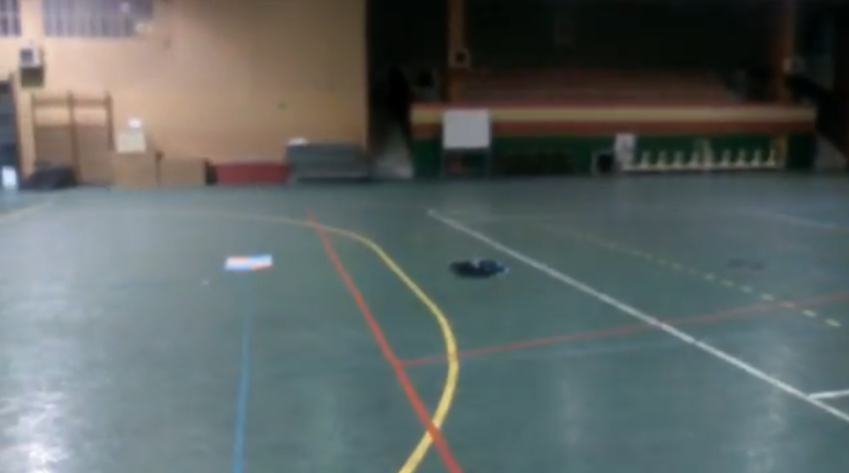
\includegraphics[width=0.33\textwidth]{imgs/complete1.png}}
  \subfloat[Despegue]{
   \label{f:Despegue}
    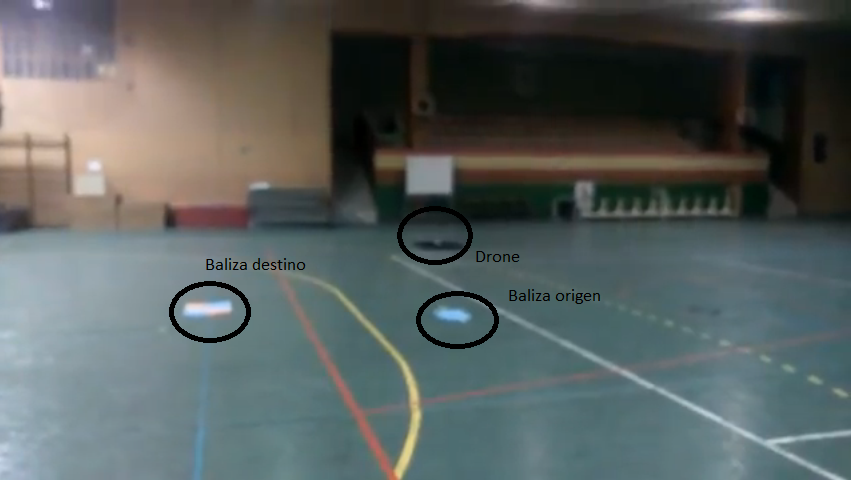
\includegraphics[width=0.33\textwidth]{imgs/complete2.png}}
  \subfloat[Despegue]{
   \label{f:Despegue}
    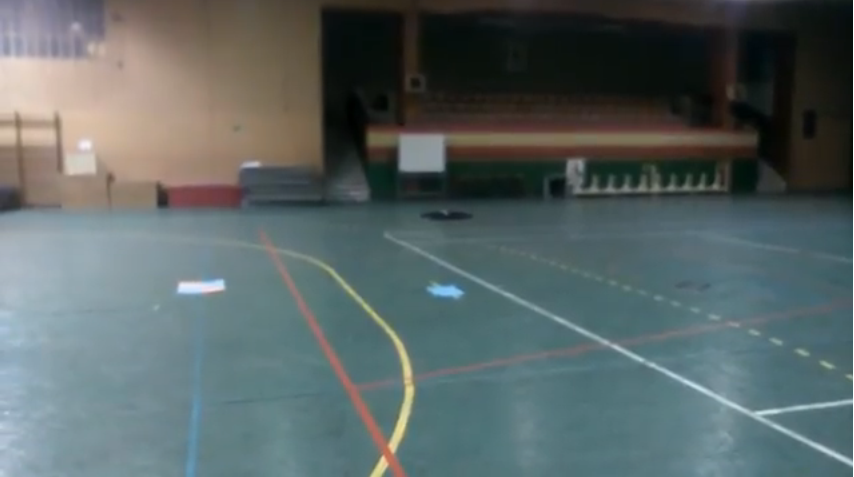
\includegraphics[width=0.33\textwidth]{imgs/complete3.png}}\\
  \subfloat[B\'usqueda]{
   \label{f:Busqueda}
    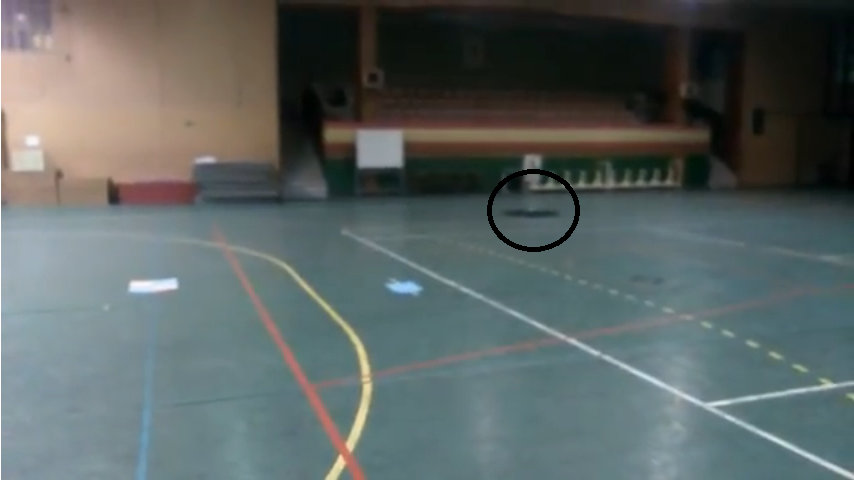
\includegraphics[width=0.33\textwidth]{imgs/complete4.png}}
  \subfloat[B\'usqueda]{
   \label{f:Busqueda}
    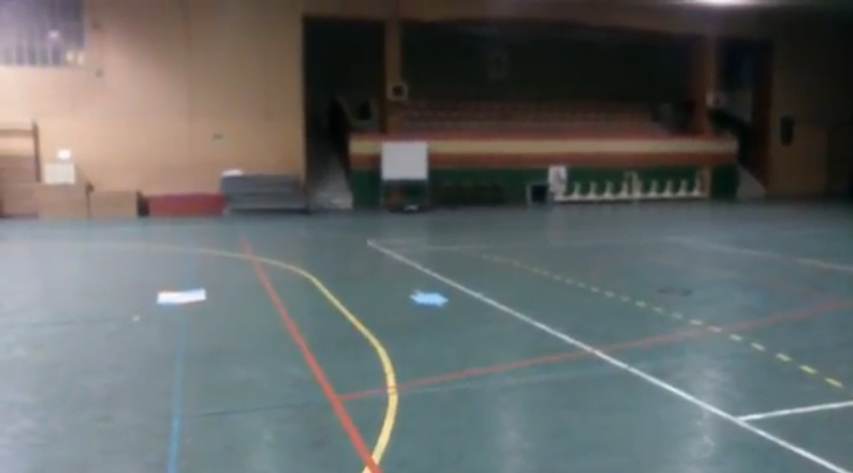
\includegraphics[width=0.33\textwidth]{imgs/complete5.png}}
  \subfloat[B\'usqueda]{
   \label{f:Busqueda}
    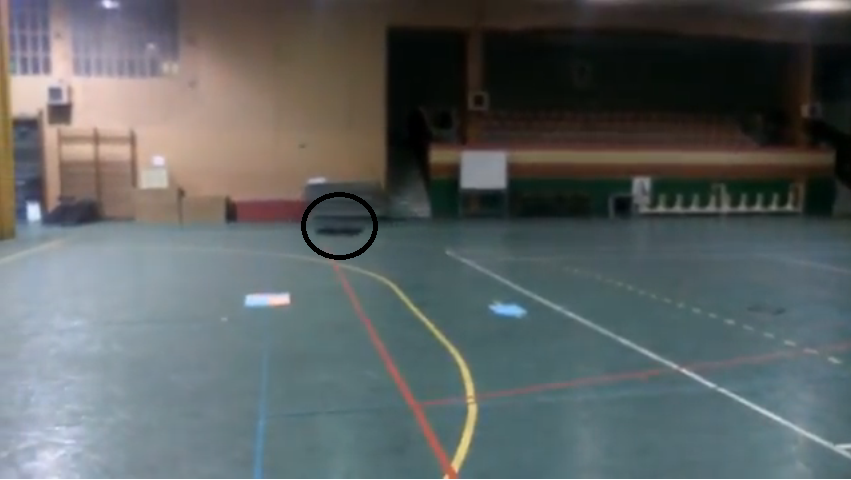
\includegraphics[width=0.33\textwidth]{imgs/complete6.png}}\\
  \subfloat[B\'usqueda]{
   \label{f:Busqueda}
    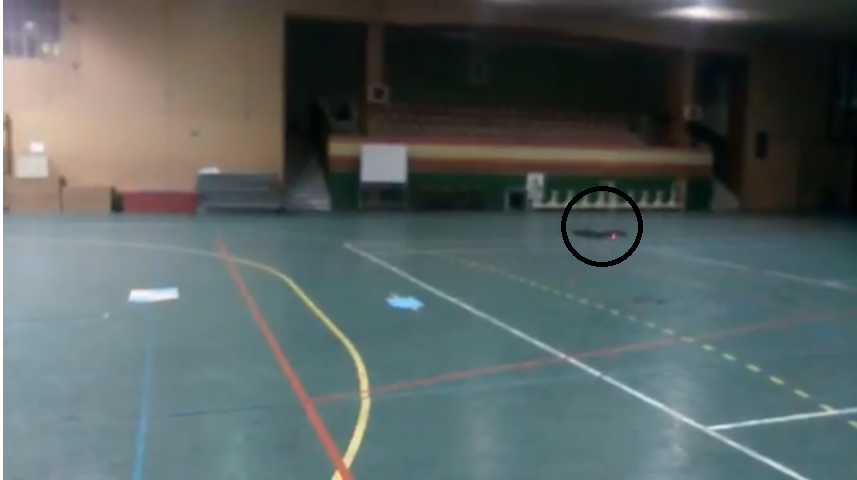
\includegraphics[width=0.33\textwidth]{imgs/complete7.png}}
  \subfloat[B\'usqueda]{
   \label{f:Busqueda}
    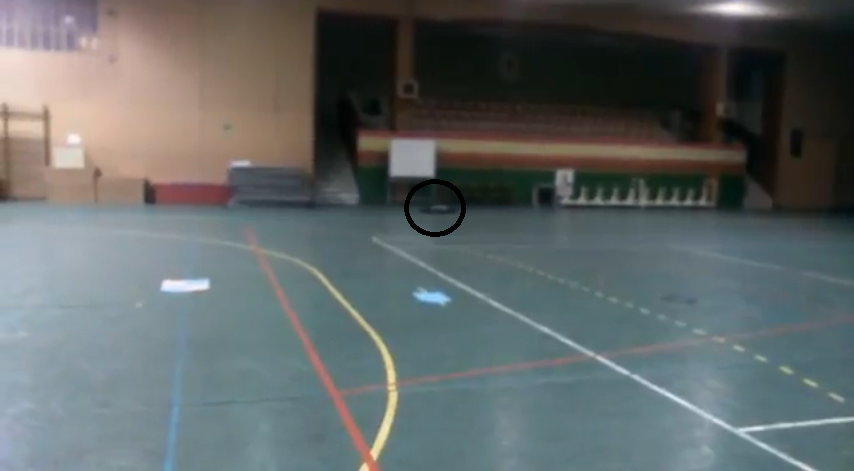
\includegraphics[width=0.33\textwidth]{imgs/complete8.png}}
  \subfloat[Aterrizaje]{
   \label{f:Aterrizaje}
    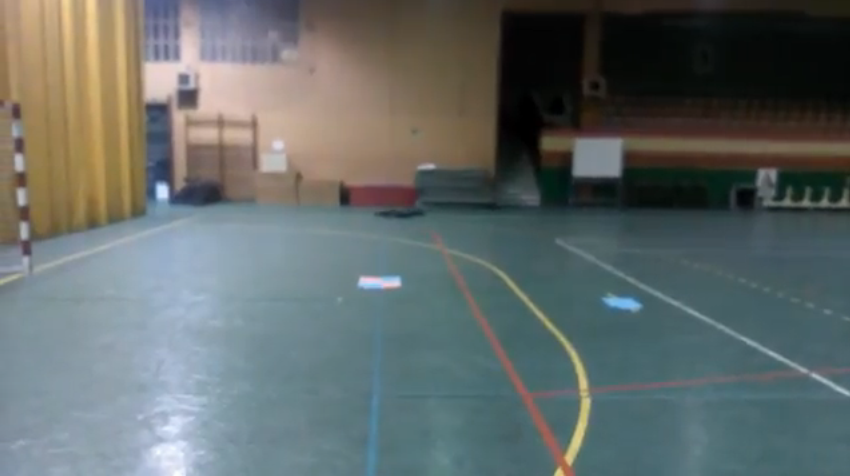
\includegraphics[width=0.33\textwidth]{imgs/complete9.png}}\\
  \subfloat[Aterrizaje]{
   \label{f:Aterrizaje}
    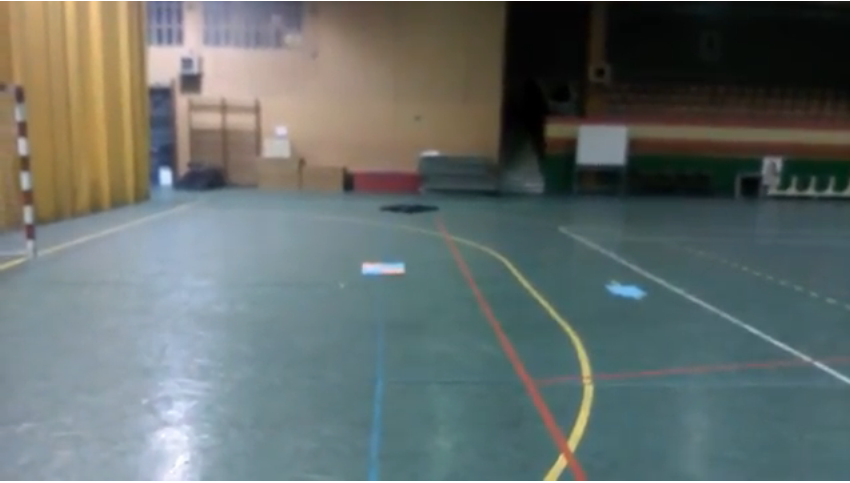
\includegraphics[width=0.33\textwidth]{imgs/complete10.png}}
  \subfloat[Aterrizaje]{
   \label{f:Aterrizaje}
    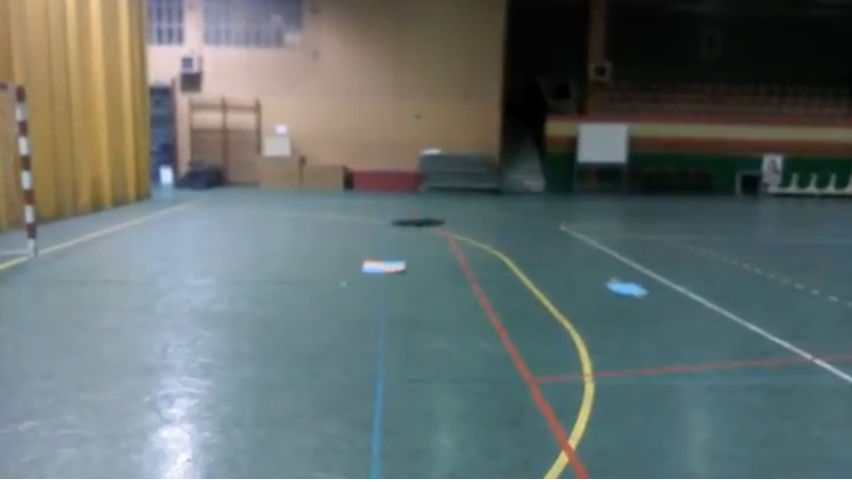
\includegraphics[width=0.33\textwidth]{imgs/complete11.png}}
  \subfloat[Aterrizado]{
   \label{f:Aterrizado}
    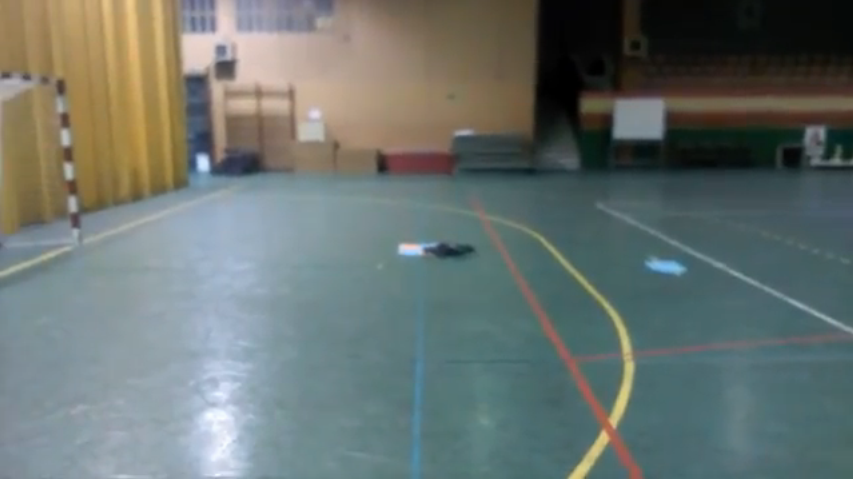
\includegraphics[width=0.33\textwidth]{imgs/complete12.png}}
 \caption{Algoritmo completo sobre el drone real. }
 \label{f:Algoritmo completo sobre el drone real. }
\end{figure}








